\chapter{Races}
\label{sec:Races}

\section{Introduction}

The people of Aror make up a multi flavoured stew of various races and
backgrounds. Apart from many races that you might be already familiar with,
such as humans, elves, dwarves or gnomes; Aror is also home to some you might
have never heard of before. Two of these are the \emph{deepkin}, the
\emph{diarim}, \emph{gorgons} and the \emph{umgeher}.

You will find that race matters little. An elf of \nameref{sec:Norbury} often
shares the warrior culture, and faith in the meritocratic societal ideas
of \emph{Norbury} much like any human. While a dwarf of \emph{Nen-Hilith} will
be accustomed and to the artistic culture and creative ways of the artisans
and performers of that city.

The union of non-humanoid races with humanoid races is something that does
not exist in \emph{Everblack}. Although you might have met ``dragonborn''
(the unity of a human and a dragon) in other realms, you will not find them
on Everblack. And if you do, they are probably extra-planar visitors much
like yourself.

\begin{note}
These sections enhance or change the existing core races of D\&D. Any lore you
find in the base books that does not interfere with what is written here, still
holds true.
\end{note}

\section{Character Races}
\label{sec:Character Races}

\begin{figure*}[ht!]
    \centering
    \vspace{-2.6cm}
    \centerline{
        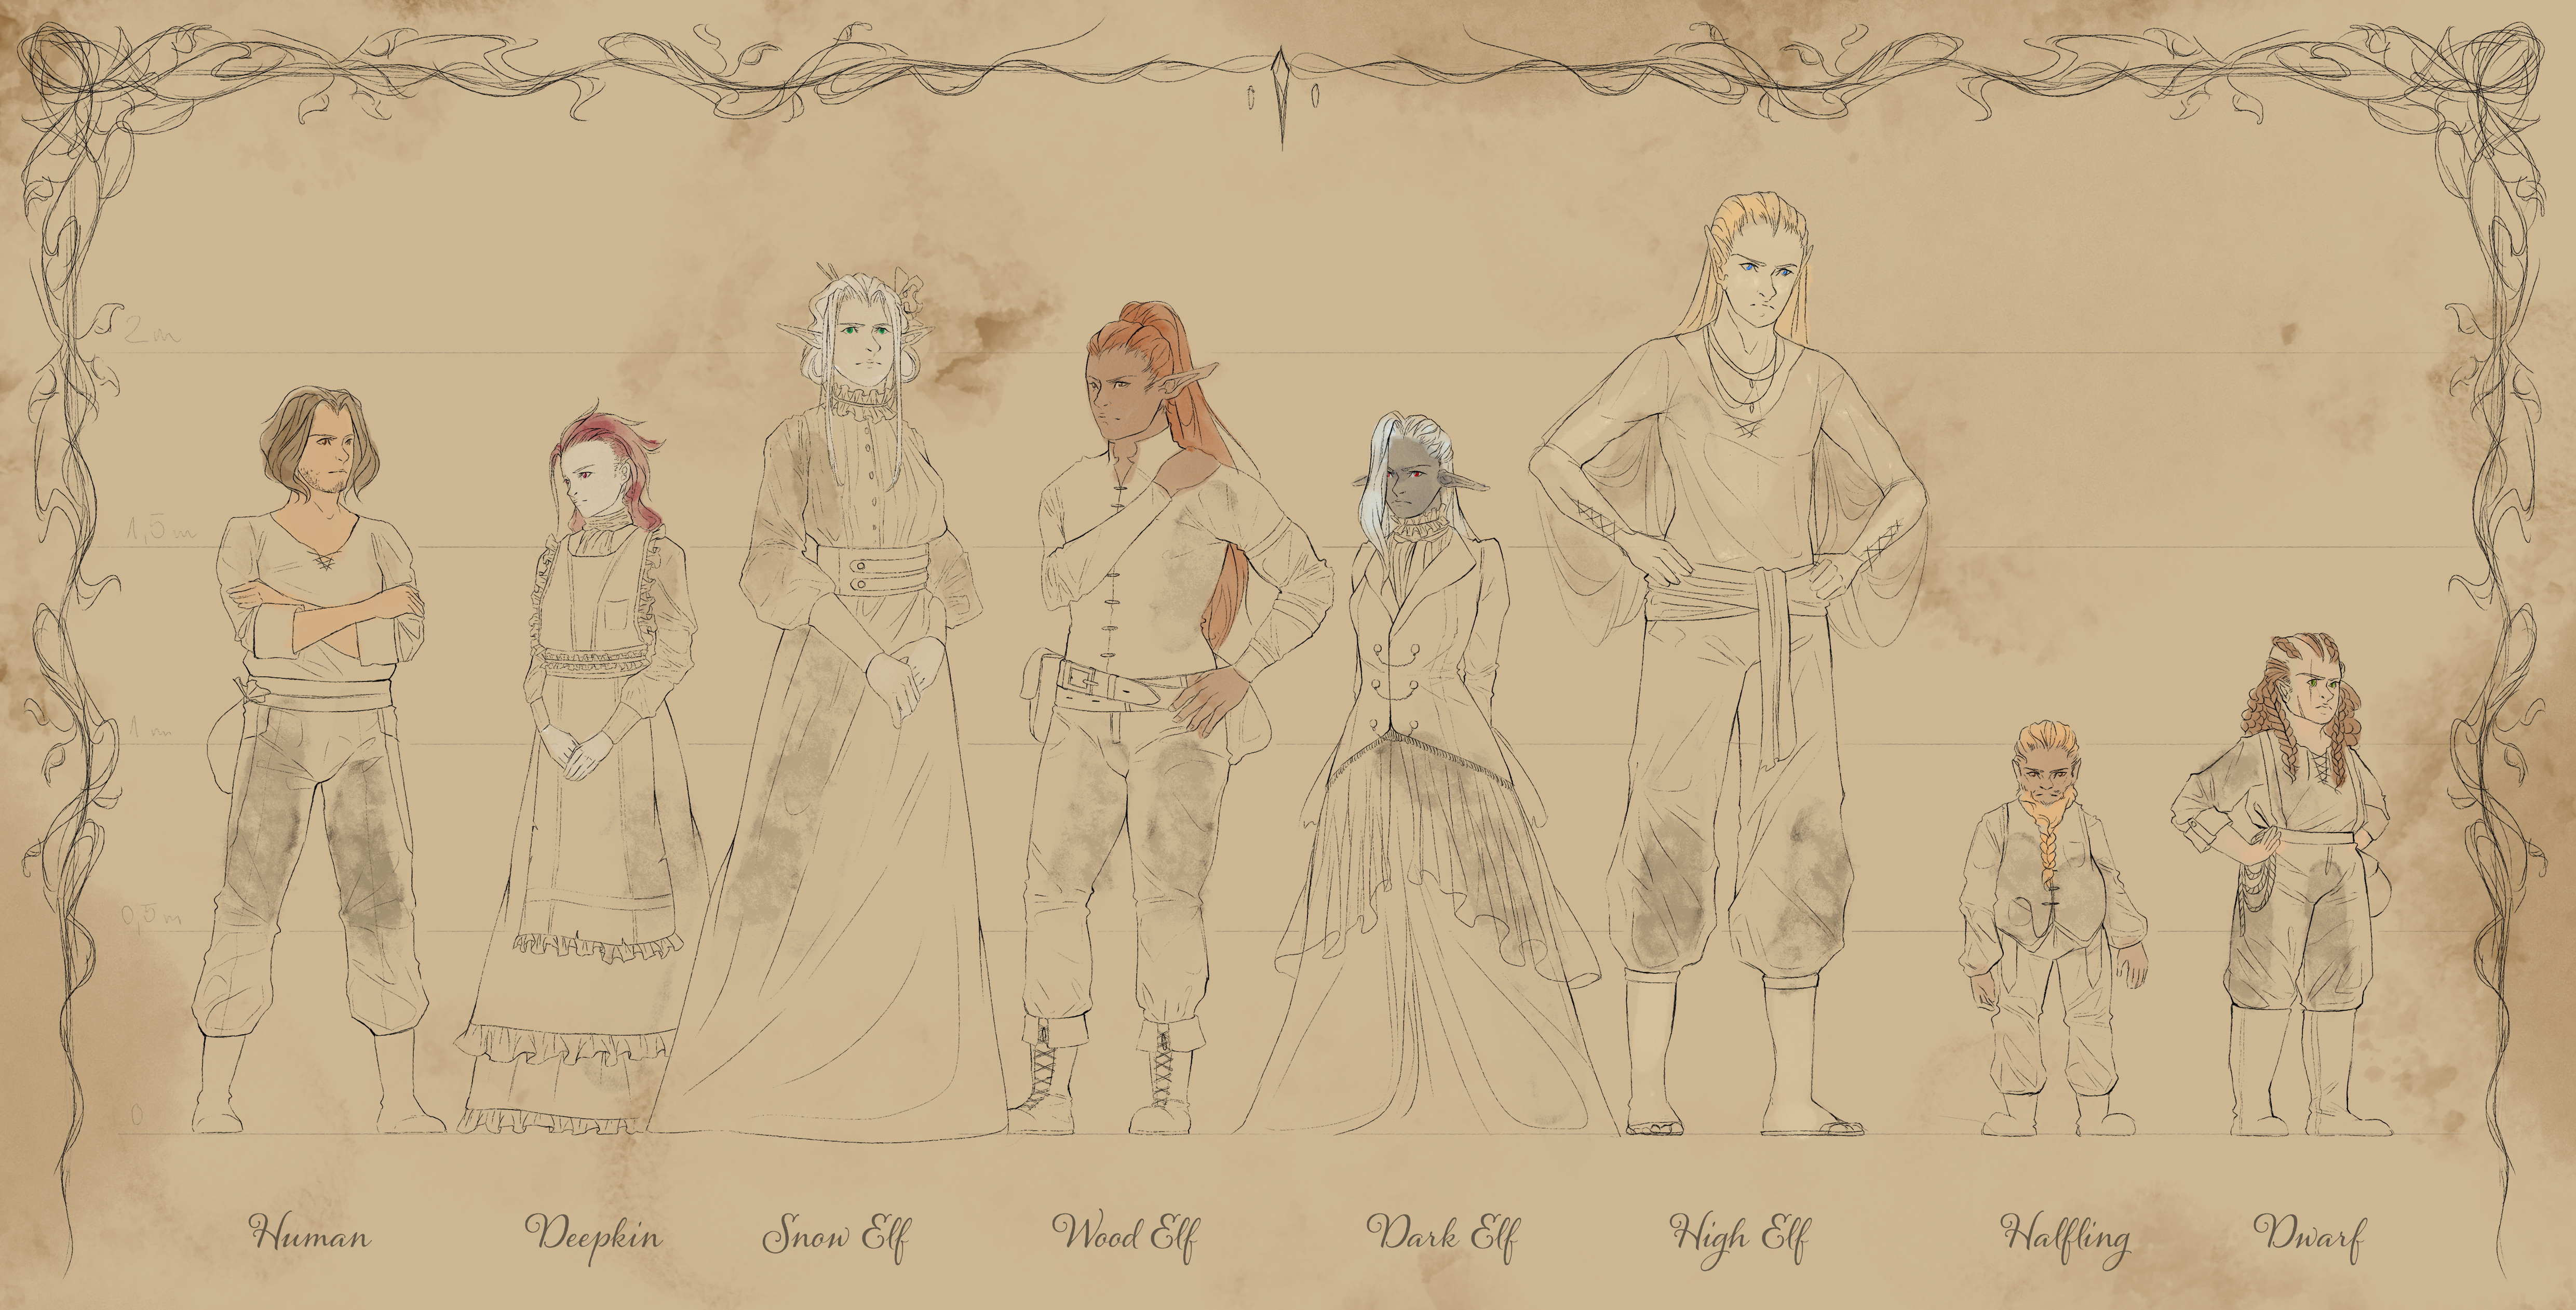
\includegraphics[width=\paperwidth,keepaspectratio]{media/coreracessm.png}
    }
    \par
    Core humanoid races of Aror: humans, elves, dwarves and halflings.
\end{figure*}

\subsection{Deepkin}
\label{sec:Deepkin}

\aren{I had the misfortune of seeing my people's decline with my own eyes.
I was powerless, and unable to stop it. We are but a shadow of our former
selves...}

\graham{But still you live. And once the time is right, you may reclaim what
once was.}

The \emph{deepkin} are the cavern dwelling cousins of humans. They are capable
of seeing in the dark (albeit without perceiving colour), and often have white
pale skin, red to brownish hair, and either red, green, blue or yellow eyes.

Deepkin society is one of the older societies on \emph{Aror}, with a long
standing history in the arcane arts, building magnificent underground cities,
libraries and workshops. Ancient deepkin were master arcane smiths, golem
constructors, inventor of many magic based constructs and technology still
used today.

The ancient deepkin had their dominance challenged by the other races of the
deep, namely the dwarves, dark elves, and a now almost extinct species called
the \nameref{sec:Ilians}. Hundreds of years of conflicts lead to the decline
of most of their impressive civilisations, with one exception. Instead of
perishing however, most of them fled to the surface, where they were warmly
received by their surface cousins. Nowadays deepkin culture is but a shadow of
what it was, although they still try to reclaim what was once theirs with
expeditions into the deep. Albeit they were well known city and kingdom
builders, only one deepkin settlement rose to the rank of a formidable city
kingdom: \emph{Stenheim}.

Although deepkin are treated as their own race, they are still capable of
producing viable offspring with normal humans. The race of the offspring is
always that of the mother, due to the dominant genetic traits of the deepkin.

\begin{35e}{Deepkin Traits}
  \hyperref[sec:Speak Language]{Doresh} is the natural language of the
  Deepkin, and is equivalent to \emph{Undercommon}.

  \begin{itemize}[noitemsep]
    \item Medium: as medium creatures, \emph{Deepkin} have no special bonuses or
    penalties due to their size.
    \item \emph{Deepkin} base land speed is 30 ft.
    \item For all manners regarding racial restrictions or classifications
    \emph{Deepkin} count as humans.
    \item Dark vision out to 120 feet.
    \item Bonus Feat: Just as their human cousins, \emph{Deepkin} can choose a
    bonus feat at first level.
    \item Automatic languages: Doresh, Teranim. Bonus Languages: Any (except
      secret languages)
    \item Favoured Class: Any. When determining whether a multi class takes an
    experience point penalty, his or her highest-level class does not count.
  \end{itemize}
\end{35e}

\subsection{Diarim}
\label{sec:Diarim}

\aren{The expression ``explaining freedom to a Diarim'' has become ingrained
  in many cultures as a metaphor for a fruitless labour.}

The \emph{Diarim} are a race of humanoid creatures that were bred for specific
tasks by the the giants living on the continent of \nameref{sec:Farlar}. They
are the youngest of the races on \emph{Aror}, and are a mixture of various
other humanoid races.

Diarim come in in as many shapes and sizes as the giants had uses and tasks
for their engineered slave race. But most share a common set of features: the
light, fair skin (almost white) of the \hyperref[sec:Deepkin]{Deepkin}, blue
hair of the \hyperref[sec:Snow Elves]{snow elves}, and an ingrained sense of
duty and loyalty to strict hierarchies from the dwarves. Almost all have blue
tribal tattoos all over their body, which identify the current and past owners
of the individual diarim. Diarim live up to 50 years, with many not living
past 30.

Very few diarim ever escape the slavery of their masters. The biological
engineering, and an ingrained culture of servitude and strong sense of
community keeps them complacent and confined within the giant culture. Diarim
were engineered to serve, do heavy labour and die as warriors on battlefields,
and thus often only strife in societies strongly leaning towards
collectivism. Diarim also all have a strong psychological need to establish
order, and they are often psychologically compelled to bring order into chaos,
reorganise, optimise or simply clean spaces they deem dirty, filthy or to be
in disarray. Most tribal diarim have no names, and they never refer to
themselves with names, and are only being given a names by the giants if they
have distinguished themselves, either through heroic deeds, or through crimes.

The most common variant are labourers, small but stout breed, that was created
by introducing more dwarven heritage into the diarim. They excel at physical
labour, such as mining and construction. Siegers were bread with monstrous
races, often even giants, and are used as front line soldiers, gladiators and
shock troops. They are larger than any other diarim, and often also serve as
overseers over other Diarim. Exciters were bred and selected for their beauty,
and are priced possessions to be traded and gifted to other giants. Their
primary role is to entertain their overlords through song, dance and company.
Exciters are also diplomats to other humanoid or monstrous nations and parties.

In the recent decades more and more diarim have escaped the continent of
Farlar and joined the other humanoid races. The giants had to learn that you
cannot suppress the curiosity, love for wandering and freedom for long when
you create a species based on humans, halflings and elves.

\begin{35e}{Diarim Traits}
  \textbf{Diarim Traits (EX)}:
  \begin{itemize}[noitemsep]
    \item Medium: as medium creatures, diarim have no special bonuses or
    penalties due to their size.
    \item A diarim's base land speed is 30 ft.
    \item \textbf{Weak Will (EX)}: All diarim have a -2 penalty to will
    saves against charms and similar effects.
    \item Automatic languages: Giant, Teranim
    \item Favoured Class: Any. When determining whether a multi class takes an
    experience point penalty, his or her highest-level class does not count.
  \end{itemize}

  \textbf{Sieger Traits (EX)}: the following traits are in \emph{addition} to
  the diarim traits, except when noted otherwise.
  \begin{itemize}[noitemsep]
    \item Large size. -1 penalty to Armour Class, -1 penalty on attack rolls,
    -4 penalty on Hide checks, +4 bonus on grapple checks, lifting and
    carrying limits double those of Medium characters.
    \item Space/Reach: 10 feet/5 feet
    \item +8 Strength, -2 Intelligence, -2 Charisma, -2 Wisdom
    \item Favoured Class: Barbarian
    \item Level Adjustment: +1
  \end{itemize}

  \textbf{Exciter Traits (EX)}: the following traits are in \emph{addition} to
  the diarim traits, except when noted otherwise.
  \begin{itemize}[noitemsep]
    \item -2 Strength, -2 Constitution, +4 Charisma
    \item Favoured Class: Bard, Sorcerer
  \end{itemize}
\end{35e}

\subsection{Dwarves}
\label{sec:Dwarves}

\emph{Dwarves} are a race of short humanoid species, belonging to four core
races that left \nameref{sec:Arania} several millennia ago. By nature dwarven
are smaller than the other races. Their stout physique lends them to tasks that
require prolonged endurance, and are thus natural labourers, and warriors.
Much like their closely related core humanoid cousins, most dwarves enjoy
living with the other core humanoid races in large kingdoms, cities, and
towns.

The dwarves that still remain in the depths are often not as open, welcoming
and tolerant. These dwarven tribes have survived the harsh realities of the
deep by creating a strictly ordered society based on castes. The clans of the
deep might be slow to trust foreigners, reclusive, isolationists, or outright
xenophobic. This culture a foundation of the the kingdom of
\nameref{sec:Kesmar}, which was founded by an isolationist, and xenophobic
tribe of dwarves millennia ago. Such dwarven cultures are only a fraction of
the living dwarven population however, and the vast majority of them live
happily together with their brethren.

\begin{35e}{Dwarf Traits}
  \emph{Rutari} is the language that dwarves of the deep speak, and is also
  the language of \nameref{sec:Kesmar}. It has its own alphabet, which is
  also called Rutari.

  \begin{itemize}[noitemsep]
    \item Medium: As Medium creatures, dwarves have no special bonuses or
      penalties due to their size.
    \item Dwarf base land speed is 20 feet. However, dwarves can move at this
      speed even when wearing medium or heavy armor or when carrying a medium or
      heavy load (unlike other creatures, whose speed is reduced in such
      situations).
    \item Dwarves are sturdy and hardy, and thus have a +2 racial bonus to
      constitution.
    \item Stability: A dwarf gains a +4 bonus on ability checks made to resist
      being bull rushed or tripped when standing on the ground (but not when
      climbing, flying, riding, or otherwise not standing firmly on the
      ground).
    \item Languages: Rutari, Teranim. Bonus Languages: Any (except secret
      languages)
    \item Favoured Class: Any. When determining whether a multi class takes an
          experience point penalty, his or her highest-level class does not
          count.
  \end{itemize}
\end{35e}

\subsection{Elves}
\label{sec:Elves}

Elves are tall - often between 1.8 and 2.4 metres - and slender race, with
long and pointy ears. The style of the elven ears varies, with some having
smaller pointy ears facing backwards, while others have longer and sharper
ears that follows the contours of their face. The variety within the elven
ears is vast, but is but a minor cosmetic difference. Their physique and build
is slender as well, with long skinny legs and arms. Elves live up to 400 years
of age, and thus often pick up professions that take longer to master, such as
wizardry, artistry or the sciences. Although elves live long, they often shift
focus in their goals. Apart from the humans, the elves are one of the older
races of \emph{Aror}.

Unlike humans, elves do have distinct sub races that differ from each other in
various physical and biological aspects. The \emph{snow elves} for example
have a natural resistance to cold like no other species have, while the
\emph{dark elves} have adapted to see better in the dark caverns they
inhabit. However they have not diverged so far from one another to not produce
vialable offspring. As with humans and deepkin the race of the sibling always
resembles that of the mother.

There are four major elven races that are recognised across the world of
\emph{Everblack}:

\subsubsection{High Elves}
\label{sec:High Elves}

The most numerous race of the elves are the \emph{high elves} of
\nameref{sec:Avenfjord}. High elves have fair skin with a hint of yellow and
gold. Their hair ranges from blond, fiery red to brown and black. They stand
between 1.8 and 2.4 metres high, towering with their slender appearance over
most other humanoid races with ease. They have pointed, elongated ears which
often point skyward, following the slender contour of their face.

High elves are the most adaptable and curious of the elves, and often live
within human city kingdoms, mixing and integrating well with other cultures
and societies. Even though they have their own kingdom, the vast majority of
high elves live outside the kingdom of Avenfjord. High elves are the only
kingdom building elven race, but do prefer to live with together with their
distant human cousins within baronies, kingdoms and city states.

The high elves are also the longest living of all the elven races, usually
living to grow 400 years old. This gives them ample time to study and learn
several fields and areas of expertise during their early childhood.

High Elves speak \hyperref[sec:Speak Language]{Enro'ad}, a variant of
\emph{Old Teranim}, but use the Taavid, halfling alphabet called \emph{Taavid}
to write it.

\begin{35e}{High Elf Traits}
  \hyperref[sec:Speak Language]{Enro'ad} is elvish, albeit the elven alphabet
  is now written with Taavid the \emph{halfling} script.

  \begin{itemize}[noitemsep]
    \item Medium: As Medium creatures, elves have no special bonuses or
    penalties due to their size.
    \item Low-Light Vision: An elf see twice as far as a human in starlight,
    moonlight, torchlight, and similar conditions of poor illumination. She
    retains the ability to distinguish colour and detail under these
    conditions.
    \item Elvish adulthood lasts longer than in other species, and they thus
      have more time to learn while they grow up. This grants them a +2 bonus
      to intelligence, and elves can select one extra
      \hyperref[sec:Education Feats]{education feat} at level 1.
    \item Automatic languages: Enro'ad, Teranim. Bonus Languages: Any (except
      secret languages)
    \item Favoured Class: Any. When determining whether a multi class takes an
    experience point penalty, his or her highest-level class does not count.
  \end{itemize}
\end{35e}

\subsubsection{Dark Elves}
\label{sec:Dark Elves}

The \emph{dark elves} live mostly underground, have black to blue skin, and
their hair ranges from a faint hint of blue, silver to snow white. Their eyes
are often red, blue or a green. They are the smallest of all elven races, and
range from 1.60 to 1.90 metres in height. In terms of bodily physique they
also more closely resemble humans. Their rounder faces, and their stronger and
more muscular physique sets them apart from their slender high elven cousins.

Dark elves once followed the dwarves underground, when the ancient battles
against the sentient non-humanoid creatures and the fey turned deadly and
dangerous. They have since adapted to that life underground, both physically
and culturally. They can see well in the dark, and their skin turned dark
letting them blend in with the dark surroundings of the depths. They also only
live roughly 120 years, and are thus not as long lived as their high elven
cousins.

Underground they are often live primitive, nomadic lives, adapted to the harsh
realities of the depths below. They have survived the dangerous environment of
the deep caverns by remaining on the move or by hiding from threats. They
value their small communities and family above all else.

Many dark elves also live on the surface, and much like their surface cousins,
they prefer to integrate into already existing humanoid kingdoms and baronies.
Dark elves are rather common all over the world, and can be found on almost all
continents.

\begin{35e}{Dark Elf Traits}
  \textbf{Dark Elf Traits (Ex)}: The following traits are in \emph{addition}
  to the high elf traits, except when noted.
  \begin{itemize}[noitemsep]
    \item Dark elves are considered smaller and more nimble than the other
      elven races, and thus gain a +2 racial bonus to dexterity.
    \item Dark vision out to 120 feet, albeit they are colour blind.
    \item Automatic languages: Doresh, Enro'ad, Teranim. Bonus Languages: Any
      (except secret languages)
  \end{itemize}
\end{35e}

\subsubsection{Snow Elves}
\label{sec:Snow Elves}

\aren{Snow Elves are the pinnacle of beauty...}

Far to the north and south live the \emph{snow elves}, nomadic hunter-gatherer
elves with white to silver blue skin, white, silver, grey or blue hair. Their
eyes are often bright blue, green or yellow. Male snow elves are capable of
growing facial hair, while many female snow elves have light red freckles
in their faces. Snow elves are as tall as their high elven brethren, ranging
from 1.8 to 2.4 metres, and also share most of their facial features with high
elves. They have adapted well to the colder climates, and can withstand the
cold far easier than any other humanoid race. This has also come with a major
drawback: With a life expectancy of 80 years, they are the elven race with
shortest lifespan. Many \emph{snow elves} live in smaller families and tribes,
content with surviving the harsh realities of the polar north and south by
becoming fierce hunters, fishers or even raiders themselves.

These snow elves from northern and southern tribes are generally known to be
calm, and quiet, preferring the solitude of a small group or town over the
vast masses and stretches of cities. They rarely leave the frozen north and
south, and are thus exotic, as in, many other humanoids haven't seen a tribal
snow elf in person. They do not build cities or kingdoms, but smaller tribes
often join to form larger ones (several hundred individuals) if required.

To tribal snow elves the community, family and their own tribe is everything, as
it ensures survival and in the frozen tundras. The harshest punishment within
these communities, reserved for major crimes, is exile which is often equal to
a death penalty. Since these exiles are then also shunned by other snow elven
tribes, they sometimes wander away from their homes and join city kingdoms or
baronies.

Snow elves rarely leave their icy domain and tribal lives willingly, and thus
the ancestors of the snow elves in the city kingdoms were either exiles, or
were once captured and brought there as slaves. Those civilised snow elves do
not harbour any animosity any more about what happened to their ancestors
thousands of years ago, and prefer to remain in the places and cultures they
now call their homes. To the tribal snow elves these city snow elves are equal
to exiles, and are thus not welcome in the frozen north or south.

\begin{35e}{Snow Elf Traits}
  \textbf{Snow Elf Traits (Ex)}: The following traits are in \emph{addition}
  to the high elf traits, except when noted.
  \begin{itemize}[noitemsep]
    \item \textbf{Pale Wastes (Su)}: A pale elf can live comfortably in
      conditions of extreme cold, even with barely any clothing or external
      sources of warmth. This ability functions like a continuous \emph{Endure
      Elements} but for cold conditions only.
    \item Snow elves are known for their great hunting skill which allows them
      to perceive hidden things and small details, and thus have a +2 bonus to
      wisdom.
    \item Automatic languages: Enro'ad, Teranim. Bonus Languages: Any (except
      secret languages)
  \end{itemize}
\end{35e}

\subsubsection{Wood Elves}
\label{sec:Wood Elves}

Wood elves have light brown or greenish skin, and green or red hair. Their
faces are often covered in light or red freckles, and their eyes are often
brown, blue or green. They are as tall as their high elven counter parts,
often ranging from 1.9 to 2.4 metres, and also share the facial features of
the other high elves. Although they are very close to their high elven
cousins, they are counted as their own race based on their ability to easily
build muscle mass. This often makes them the strongest elven race, and a wood
elf can easily be compared to \nameref{sec:Half-Orcs} in terms of bodily
strength. Even though they are known to join the major city kingdoms, they are
rarer than high or dark elves.

There are two major communities of wood elves. The first lives in the vast
temperate and boreal forest of \nameref{sec:Eilean Mor}, known as the
\nameref{sec:Dirgewood}. These wood elves live together with humans, halflings
of the Dirgewood, as well as the dark elves, deepkin and the dwarves of the
\nameref{sec:Great Divide}. They are followers of the \nameref{sec:Old Ways},
and prefer to build small settlements, towns and perhaps tiny cities of their
own. These wood elves are expert trackers, hunters, farmers, as well as shamans
and priests of the old ways.

And in the jungles \nameref{sec:Yuacata} live the \emph{savage elves}, a loose
collection of tribes of cannibalistic and demon worshipping wood elves. They
rarely wander beyond the confines of their jungle and are one of the rarest
elven culture to meet in the civilised areas of \emph{Aror}. They live a
primitive life, adapted to the harsh and dangerous rain forest.

\begin{35e}{Woold Elf Traits}
  \textbf{Wood Elf Traits (Ex)}: The following traits are in \emph{addition}
  to the high elf traits, except when noted.
  \begin{itemize}[noitemsep]
    \item Wood elves have it easier to gain muscle mass than the other elvish
      races, and thus have a +2 racial bonus to strength.
    \item Automatic languages: Enro'ad. Bonus Languages: Any (except secret
      languages)
  \end{itemize}
\end{35e}

\subsection{Gnomes}
\label{sec:Gnomes}

\emph{Gnomes} are the children of \emph{halflings} and \emph{dwarves}. Since
they have no identity of their own, no culture of their own, they often try to
integrate with their parents' cultures. Albeit they rarely fit in with either
societies. Gnomes themselves are sterile, and thus rarely settle down to found
their own families. This often leads them on a live of adventure, discovery or
studies of the sciences or arcane arts. They have inherit the longevity of
their dwarven parents, as well as their short stature. All in all \emph{gnomes}
are among the rarest races on \emph{Aror}.

There are no \emph{gnome} settlements or even kingdoms, and most of them live
scattered across the world in the large city kingdoms. Offering their services
as spies, thieves and adventurers to anyone willing to pay. Most large dwarven
cities and halfling settlements also have a small \emph{gnome} population.

\begin{35e}{Gnome Traits}
  \begin{itemize}[noitemsep]
    \item Small: As a Small creature, a gnome gains a +1 size bonus to Armor
    Class, a +1 size bonus on attack rolls, and a +4 size bonus on Hide
    checks, but he uses smaller weapons than humans use, and his lifting and
    carrying limits are three-quarters of those of a Medium character.
    \item Their dwarven blood makes them hardier and sturdier, and thus have
      a +2 racial bonus to constitution.
    \item Gnome base land speed is 20 feet.
    \item Low-Light Vision: A gnome can see twice as far as a human in
    starlight, moonlight, torchlight, and similar conditions of poor
    illumination. He retains the ability to distinguish color and detail under
    these conditions.
    \item Languages: Teranim, Rutari. Bonus Languages: Any (except secret
       languages)
    \item Favoured Class: Any. When determining whether a multi class takes an
    experience point penalty, his or her highest-level class does not count.
  \end{itemize}
\end{35e}

\subsection{Gorgons}
\label{sec:Gorgons}

\emph{Gorgons} are a half-breed between any of the three medusa races, and a
humanoid father. Since medusa have no males, they must rely on other monstrous
or humanoid races to reproduce. The birth of a gorgon is rare, and most children
between a medusa and a humanoid father results in a pure breed medusa of the
same type as the mother.

Much like their mothers' race, gorgons are a female-only species. They inherit
their humanoid appearance - such as physique, build, skin, ``hair'' or eye
colour - from their father, but gain certain traits from their mothers. Just
like medusas, gorgons have small snakes as hair upon their heads. Areas where
the skin on humanoids is harder and tougher - like on the elbows and knees -
Gorgons have patches of reptile scales instead. From afar a gorgon passes as
normal humanoid female, and thus many gorgons hide their ``hair'' with
clothing or even disguise spells to pass as humanoids.

They inherit the ability to turn people into stone from their mothers, but
the power of the effect is weaker. Still gorgons must actively avoid looking
other people in the eyes or risk turning them to stone permanently. Any other
special traits (such as wings, another set of arms etc.) are not passed down
to Gorgons.

There are two main variants of Gorgons: The most common variant has the heads
of snakes as hair, while the others have the tails of snakes as hair. The
snakes and the gorgon live in a symbiosis together, and a Gorgon can feel
any sensation or pain that the snakes experience. Those gorgons with snake heads
can also perceive the world through the eyes of the snakes. They do not
directly see through the eyes of their snakes, but the snakes make them
indirectly aware of their surroundings. A snake's bite is not venomous, and
the snakes collectively also reflect the gorgons mood and feelings. Anyone who
knows a gorgon well can deduce the mood from the snakes' behaviour, even if
she tries to hide it her true feelings. Those gorgons with snake tails have
fine motor control over their ``hair'', and can use them to carry, use and
manipulate light objects on a fine scale.

Gorgons almost always leave medusa society, and try to integrate into the
societies of the father's side. They then often attempt to fit in with the
other humanoids, but are met there with superstition and fear. Still many
gorgons grow up in humanoid societies, and thus share many aspects, values and
traits of the culture they grew up in. Generally gorgons are known to be kind,
adventurous, open minded, as well as excellent scholars, bards and wielders of
the arcane arts. Still many societies do not allow Gorgons, or only those that
cover their eyes, out of fear of the damage they might inflict on others.

\aren{No one can be blamed really, since it is a humanoid instinct to look
  each other into the eyes.}
\graham{True. People can be crippled or even die if turned to stone in a
  position that is unbalanced, and causes the statue to fall over and break.}

\begin{35e}{Gorgon Traits}
  Gorgons speak Teranim, and whatever additional languages their culture and
  background provides.

  \begin{itemize}[noitemsep]
    \item Medium: As Medium creatures, Gorgons have no special bonuses or
      penalties due to their size.
    \item Medusa Heritage (EX): Gorgons are a female only species.
    \item Gorgons inherit their beauty and expressive personality from their
      mothers, giving them a +2 bonus to charisma.
    \item Snake Vision (EX): A gorgon with snake heads as hair can perceive
      the world even if it has been blinded. She can see and detect shapes,
      movement as well as smaller details giving her \emph{Blindsense (30
        ft.)}.
    %% Mirdon would be proud
    \item Snake Hands (EX): A gorgon with snake tails as hair can use their
      hair as an extra limb to wield, manipulate, or use small objects, such
      as wands, light weapons, or other smaller items. These snakes can also
      be used for somatic components of spells. All snakes together are
      required for these tasks, and thus the entire ``hair'' counts as one
      limb.
    \item Petrifying Gaze (SU): Turn to stone permanently, 30 feet, Fortitude
      DC 12 negates. The save DC is Charisma-based.
    \item Level Adjustment: +1
  \end{itemize}
\end{35e}

\subsection{Half-Elves}
\label{sec:Half-Elves}

The union of an \hyperref[sec:Elves]{elven} father and a
\hyperref[sec:Dwarves]{dwarven} mother produces a half breed called
\emph{half-elves}. They inherit their slender appearance from their elven
heritage, often looking beautiful, gracious and fair, and combine the
longevity of their elven and dwarven heritage to live up to 200 years. They
are well accepted by most cities and towns of the humanoid races, and often
use their elven appearance to take up jobs as entertainers, diplomats, traders
and bankers. They are known to be hard working, conscientious, intelligent and
crafty. Highly favourable traits they have gained from their dwarven
heritage. Much like with muls, the pregnancy of a half-elf can be dangerous
for the dwarven mother, sometimes leading to complications during birth. But
unlike muls, half-elves are not sterile as long as they reproduce with other
half elves.

Since very few half elves are ever born at any given time, a small but highly
dedicated community of half elves have arisen in most larger centres of
civilisation. These communities often aid and support any born half elf, even
though they rarely face any difficulties to begin with. Since the half elves
are born so rarely, and their trait is non-dominant (meaning that only the
union of two half elves produces another half elf), these communities openly
encourage marriage among their members to grow the community and the species
as a whole.

\begin{35e}{Half-Elf traits}
  The following items are in addition to the base 3.5e half-elf traits, as
  described in the d20 SRD.
  \begin{itemize}[noitemsep]
  \item Having gained the natural beauty and fairness of the elven heritage,
    they gain a +2 racial bonus to Charisma.
  \item They have inherited the craftiness of their elven parents and thus
    may select an additional \hyperref[sec:Background Feats]{background feat}
    at level 1.
  \end{itemize}
\end{35e}

\input{chapters/races/halflings}
\subsection{Half-Orcs}
\label{sec:Half-Orcs}

Less rare than \emph{Gnomes}, \emph{half-orc} are the offspring of the union
of human, deepkin or elf with an orc. Any union including an orc (either as
mother or father), will produce a half breed. They share distinct traits of
their orcish heritage, such as greenish to grey skin, large protruding
eyetooth (often dismissively called ``tusks''), and a large, towering and
muscled physique.

\emph{Half-orcs} are sterile, and thus have no inner need or desire to settle
down or start families. They often live amongst their humanoid parents
offering their brute strength and enduring physique as heavy labourers or
fighters. A human mother giving birth to a \emph{half-orc} has a change of
dying due to complications, albeit birthing a half orc is less dangerous than
giving birth to a \nameref{sec:Mul}.

And since very few women take such a risk, many \emph{half-orc} children are
not the result of a voluntary union. This sad reality, combined with a short
temper, less than flattering appearance and social hardship, often elicit
condescending or outright demeaning behaviour from the other races towards
\emph{half-orcs}.

\begin{35e}{Half-Orc Traits}
  \begin{itemize}[noitemsep]
    \item Their orcish blood makes it easier for half-orcs to gain muscle mass
      and thus have +2 racial bonus to Strength.
    \item Medium: As Medium creatures, half-orcs have no special bonuses or
      penalties due to their size.
    \item Half-orc base land speed is 30 feet.
    \item Orc Blood: For all effects related to race, a half-orc is considered
    an orc.
    \item Automatic Languages: Teranim, Orc. Bonus Languages: Any (except secret
      languages)
    \item Favoured Class: Any. When determining whether a multi class takes an
    experience point penalty, his or her highest-level class does not count.
  \end{itemize}
\end{35e}

\subsection{Humans}
\label{sec:Humans}

\emph{Humans} are one of the most prolific of the humanoid races of Aror, and
also the dominant race of the planet. Human artefacts have been found dating
back thousands of of years, outmatching the other humanoid races. There are
two separate ``races'' of humans: those inhabiting the southern part of the
hemisphere who usually have darker skin, and the ``northerners'' who usually
have fair skin. This distinction is superficial only. Apart from the tone in
skin colour, there is no other biological difference between the various human
tribes and civilisations. Humans live up to 80 years, and are known for being
statesmen, diplomats, farmers, adventurers, explorers and scientists.

Humans can be found everywhere on Aror. But history indicates that they
originated on the southern continent of \nameref{sec:Arania} together with the
other core humanoid races, and migrated to all other continents during the
last ice age twenty thousand years ago. Wherever humans settle they build
villages, cities, and large kingdoms and often become the dominant culture and
social structure. Human kingdoms have often endured for hundreds of years, and
have bested many difficulties that had driven other societies to ruin. The
ingenuity of the humans, their stubborn attitude and their uncanny ability to
adapt to any difficulty makes them the dominant race of Aror.

Like most races, humans have no inherent global culture, tradition or customs.
Instead their believes and customs are ever evolving, and specific to the
realm they live in. But there is one trait that the average human has: ingenuity
in the face of adversity. No other species has managed to settle every corner
of the world and endure, and even build lasting civilisations out of the
hostile environment they found themselves in.

\begin{35e}{Human Traits}
  \begin{itemize}[noitemsep]
  \item Medium: As Medium creatures, humans have no special bonuses or
    penalties due to their size.
  \item Human base land speed is 30 feet.
  \item 1 extra feat at 1st level.
  \item 4 extra skill points at 1st level and 1 extra skill point at each
    additional level.
  \item Automatic Language: Teranim. Bonus Languages: Any (other than secret
    languages).
  \item Favoured Class: Any. When determining whether a multiclass human takes
    an experience point penalty, his or her highest-level class does not count.
  \end{itemize}
\end{35e}

\subsection{Umgeher}
\label{sec:Umgeher}

\aren{I was once the midwife of an \emph{Umgeher}...}

\graham{The less shared about this experience the better.}

\emph{Umgeher} (old Teranim for someone who walks again) are undead humanoids
that retained their own individuality, will, memories and determination across
the process that turned them into undead. They were created centuries ago by
the ancient vampires that reign in the city kingdom of \nameref{sec:Helmarnock},
and were given the physical ability to reproduce on their own, without turning
others towards undeath.

This allowed them to establish themselves as their own species on Aror, and
thus soon travelled and spread across the entire known world. Umgeher are
neither immortal, nor are they invincible. Umgeher live to be a hundred years,
do not require food or sleep, but must drink water to survive. More so, their
flesh and skin is in a constant state of decay, and must combat their never
ending dissolution with oils, ointments or arcane spells. They have no bodily
hair, and often wear wigs to blend into normal population. Umgeher have a
distinct physiology vulnerable to damage, compared to other undead, and
require doctors to heal wounds, fix broken bones, or diagnose degrading health
at advanced ages.

Umgeher, like any species, are free to determine their own fates and shape
their own destinies. They do have to constantly combat the ignorance and fear
of the other races, but most city states have now allowed umgeher to become
full citizens, and treat them equal to any core humanoid race. This was a
recent trend however, and most umgeher prefer to build their own little
communities and towns in more rural areas.

Many religious institutions that see necromancy and undead as a defilement of
life, also persecute, hunt and destroy umgeher. Those institutions are also
to blame for the many lies that have spread across the general populace about
umgeher, such as their fanatical cravings about humanoid flesh, or that they
will take over heavy labour sectors in an economy.

\begin{35e}{Umgeher Traits}
  \begin{itemize}[noitemsep]
    \item Type: \emph{Undead}.
    \item Medium: as medium creatures, \emph{Umgeher} have no special bonuses or
      penalties due to their size.
    \item \emph{Umgeher} base land speed is 30 ft.
    \item As living undead umgeher gain all undead traits, except only gain
      partial immunity to critical attacks. This effect is equivalent to 50\%
      fortification. Umgeher follow humanoid growth cycles (i.e. are born, have
      a childhood, young adulthood, adulthood and finally seniority) and live to
      become roughly 100 years. Furthermore Umgeher must drink water like any
      living species.
    \item \emph{Umgeher} have a live long experience in disguising themselves as
      humans, and thus gain a \emph{+2 racial bonus} on \emph{Disguise} and
      \emph{Bluff}.
    \item Favoured Class: Any. When determining whether a multi class takes an
      experience point penalty, his or her highest-level class does not count.
    \item Automatic languages: Teranim. Bonus languages: Any (except secret
      languages).
    \item Level Adjustment: none
  \end{itemize}
\end{35e}


\section{Monstrous Races}
\label{sec:Monstrous Races}

\aren{For a long time I considered an honorable and noble ogre named
  Gor'esch'tar my best friend. Mothers' bless his kind soul.}

When the core humanoid races set forth from the continent
of \nameref{sec:Arania} to settle the world, they found it already inhabited
by many different monstrous races. Some of which are sentient, others even
built civilisations such as towns, cities or even kingdoms, while others are
mere beasts and animals. Monstrous races can be found on all of Aror, but are
rarer on \nameref{sec:Eilean Mor} as they have been pushed back by the
humanoid races on that continent for hundreds of years.

\subsubsection{Two Fronts}

Much like with humanoids, you will find members of the monstrous races from
all walks of life, holding many different believes, exhibiting all kinds of
attitudes, and perhaps even sharing the very same dreams and hopes that you do
as well. The only constant on Aror is the centuries old feud between monstrous
and humanoid races that finds its roots in the \nameref{sec:Aeon of
  Strife}. It has sown hatred, distrust, animosity and cost thousands, if not
millions of lives on both sides.

Even after the aeon of strife had ended, many beast races continued to raid
human settlements, entrenching the divide between the two deeper and deeper.
Hobgoblins, ogres, trolls and bugbears often sail south from the shores of
\nameref{sec:Iafandir} towards \nameref{sec:Eilean Mor}, raiding the coastal
villages and baronies for wealth, food, artefacts and slaves. This in turn
gave rise to warring nations such as \nameref{sec:Norbury} or
\nameref{sec:Morkan}, adding fuel to the hatred between the two factions.

This is often precipitated by the ever expanding humanoid settlements, who
encroach on land already inhabited by monstrous tribes and villages. Since the
city kingdoms, baronies and lordships often wield bigger military might, they
sometimes forcefully remove, exile or even kill monstrous tribes to continue
their expansion.

\subsection{Dragons}
\label{sec:Dragons}

Dragons are a race of highly intelligent, winged creatures with reptilian
traits. They come in a variety of shapes, sizes and colours. They grow bigger
and more powerful they more they age and mature.

The size of dragons ranges from small (roughly one metre), up to gigantic (20
metres), depending on their age. They have lightweight, yet protective scales
that cover most of their bodies. And their skin colour range from black, blue,
green, red white, to brass, copper, gold or silver. Dragons with more than
one colour are very rare, but have been observed as well. All dragons are
capable of breathing fire, and some even master secondary or even tertiary
elementary breath as they grow older.

The dragons of Aror are immortal but not invulnerable. Furthermore each
hatchling is born with the genetic knowledge of its two parents. This knowledge
is not immediately available to the young dragon, but is instead unlocked
over the course of decades, or even centuries, as the dragon gains new
experiences, impressions and learns about the surrounding world. Young dragons
thus study among their own adults, in an attempt to learn new things, as well as
to unlock their own hidden powers and knowledge. Dragon eggs that successfully
hatch are a rarity, and so only a few young dragons are born in a century.

Dragons, with their aeons of study of the sciences and the arcane arts, are
highly advanced engineers, smiths, and spell casters. They have made many of
the arcane artefacts that can be found on Aror, such as the
\nameref{sec:Dragon Teleporters}.

Most dragons on Aror live on a continent called \nameref{sec:Draigynus}, which
is named after them. Dragons are not a native species of Aror, and have settled
this continent after arriving on the planet from another plane. It is unknown
when, or from where they came.

In \emph{MI:1916} the \hyperref[sec:Giants]{giants} arrived on the northern
continent of \nameref{sec:Farlar}, to wage war against the dragon colony. The
dragons were joined by the halflings and elves of the city of Nen-Hilith,
until the city was destroyed by the giants. Over two hundred dragons have lost
their lives in the war, and by \emph{MI:2008} the war is still continuing.

About a hundred dragons now remain on the continent, and have organised
themselves into a small clan lead by the eldest, and most wisest of the
dragons, called the \emph{elder}. This elder is supported by an apprentice
dragon, that is referred to as the \emph{aspirant}. The dragons are known to
keep to themselves, and prefer not to mingle with what they call ``younger
races''. To them the continued existence of their rather small clan is the
utmost importance, and they will do anything to protect themselves, and
especially their young and unborn. Threatening, harming a young or unborn is
the worst crime anyone can inflict in dragon society, is punishable by death.

Although the dragons have no use for gold or money, they have began hoarding
wealth by selling or trading arcane weapons, armour and artefacts to the
humanoid races. In exchange humanoid and monstrous mercenaries fight for them,
deepkin and dwarven engineers build siege engines and golems, and elven and
halfling raiders strike their old homeland in daring raids to cripple the
efforts of the giants.

\begin{35e}{Dragons}
  Overall dragon society is considered \emph{neutral good}, albeit you can
  find dragons ranging in all sorts of alignments.

  All dragons breath fire foremost, and once they reach the \emph{young adult}
  stage of development (so after 50 years of age) they gain the ability to
  breath another element. A \emph{mature dragon} (200 years or older) gains a
  tertiary element. Roll these at random from the list of available elements:
  \textbf{acid}, \textbf{sonic}, \textbf{electricity}, \textbf{cold}, or
  \textbf{force}. The dragon can decide which form the breath attack takes,
  before the attack as a free action. The dragon also gains immunity against
  the elements it breathes.

  Dragons gain no spell-like abilities, but all dragons gain the \emph{Water
    Breathing} extraordinary ability.
\end{35e}

\subsubsection{Fey}
\label{sec:Fey}

Fey are magical and evil forest spirits that were created by the
earliest \hyperref{sec:Druids}[druids] to protect nature from
destruction. During the \nameref{sec:Strife}, both monstrous and
humanoid culture uprooted forests, cleared grassland, dried marshland or
outright destroyed or corrupted nature to fuel their war machinery and ever
growing populations.

Druids, from both sides of the war, desperate to preserve nature created
forest spirits that should serve as protectors to nature. But after the druids
realised that the gentle spirits they had created proofed ineffective in
deterring the humanoid and monstrous loggers, they used necromancy to corrupt
these spirits into evil and sadistic creatures.

The fey are now universally hated and feared, and are often the cause for
great disasters, tragedies and destruction in both humanoid and monstrous
villages and communities. Their madness has clouded their judgement, and fey
attack anyone who ventures into their forests, even druids.

The most common fey are \emph{red caps}, small vicious and sadistic
human-like creatures that hunt and murder for nourishment.

Dryads attack loggers and travellers that seek the shade of the tree they are
meant to protect. Originally created merely as a beautiful illusion to woo
loggers into leaving trees unharmed, they were soon made flesh after loggers
realised they were nothing but illusions. They feast upon living flesh, and
sacrifice all those they catch to the very tree they inhabit.

Nymphs and Irrlichter seek to lure people into a marshy death by luring them
into the forest with illusions. Nymphs, much like dryads, do so by preying on
the weaker will of men, who in the early years made up the bulk of the work
force working on uprooting forests and draining swamps.

Satyrs were made to emulate the tribal patterns of the humanoid and monstrous
races and build their own villages. From there, they venture forth to raid and
pillage other villages and towns. They are capable of forging steel, and are
expert hunters and trackers. They are often aided by evil sprites and pixies,
that support the satyrs with their inherent magical abilities. Sprites and
pixies are in turn corrupted souls and spirits.

\begin{35e}{Fey}
  Everblack fey do not vanish upon death, they simply die like any other
  mortal creature. All fey that are \emph{good}, move their alignment towards
  \emph{evil}. Most of them either serve druids unwillingly, or roam the
  forests, plains and mountains seeking wreak havoc on the monstrous and
  humanoid creatures alike.

  An \emph{Irrlicht} has the same statistics as a will-o-wisp, but are of
  type \emph{Fey} instead.
\end{35e}

\subsection{Giants}
\label{sec:Giants}

\aren{The most deadly force allowed to roam free on Aror.}

Giants are humanoid-like species that combine great strength, size, intellect
with a vicious mentality for conquering that allow them to destroy anything and
anyone that gets in their way.

Not native to Aror itself, the giants arrived in \emph{MI:1920} to the continent
of \nameref{sec:Farlar} from an unknown plane. Giants share a bloody and violent
history on other planes with \nameref{sec:Dragons}, and have thus invaded the
world in an attempt to destroy the dragon clan that has settled on
\nameref{sec:Draigynus}.

Aeons ago large clan of dragons once ruled the native home plane of the
giants, subjugating, controlling and oppressing the giants. The dragons used
the giants as soldiers in a war against daemons, and as menial labourers to
create powerful arcane artefacts and defences. The giants rebelled, killing
most of their dragon overlords, and shifting their own newly formed society
towards war, violence and a deeply ingrained hatred towards the dragons. Their
home was destroyed in the violent revolution, and now the giants roam the
habitable planes in an endless conquest to make the dragons pay for their
misdeeds.

To them it no longer matters whether a dragon was actually involved in the
subjugation of their own race. Stopping history from repeating itself by all
means necessary has become a cultural and societal obligation.

They have a reputation for being strong, violent, and highly intelligent.
Giants are expert tacticians, warriors and wielders of the arcane arts. They
rival the dragons themselves in expertise on crafting and creating arcane
weaponry, machinery and artefacts. Although an individual giant is no match
for an adult dragon, they make up their individual weakness with careful
planning and preparation in their assaults.

Although several species of giants exist (such as the shorter fire giants, or
the taller storm giants) these differences are overlooked within giant society.
They are united by two main causes: conquering new lands, and defeating their
old enemies the dragons.

Giants are expert arcane wielders, are known to be the creators of several
sentient species such as the \nameref{sec:Diarim}. Early history alludes to
the possibility that the giants arrived on Aror aeons ago in their search for
dragons, but found none. Nevertheless they settled the continents of
\nameref{sec:Eilean Mor} and \nameref{sec:Iafandir}, and were responsible for
creating some of the monstrous humanoid species such as trolls and ogres.

The giants that arrived on \nameref{sec:Farlar} were responsible for the
destruction of \emph{Nen-Hilith} the city of the elves and halfings. They are
slavers, warriors but fight only those that would join their war on the side
of the dragons.

\begin{35e}{Giants}
  All giant races (except for hill giants) gain +4 intelligence, and prefer to
  become fighters and wizards. Overall their society could be considered
  \emph{chaotic neutral} as they will consider any method viable that aids them
  in their war.
\end{35e}

\subsection{Gnolls}
\label{sec:Gnolls}

\emph{Gnolls} are a monstrous race, half-humanoid, half-hyena, that live in the
deserts of \nameref{sec:Arania}, and \nameref{sec:Goban}.

Gnolls are deeply spiritual folk, often following either an evil interpretation
of \nameref{sec:Forun}, which they call \emph{Wa'het}. Gnolls are often lead by
the wises high priestess of the tribe. They believe that the fires that Wa'het
sends are meant to test, scar, challenge and destroy those that are either too
corrupt or too weak to face her face trials. Thus most gnoll tribes hold
failure, cowardice and weakness as grave sins. They respect those that hold
wisdom, tradition and braveness as virtues.

Even though gnolls are nomadic by nature, they are the only monstrous race to
hold a city that rivals the great city kingdoms of Aror. In \emph{MI:1213} the
city kingdom of \nameref{sec:Esmayar} fell to gnoll raiders, and has sinced
flourished as a gnoll kingdom.

Smaller packs of gnolls, lead by a high priestess still roam the vast deserts,
where they often avoid direct conflict with the other races. The nomadic gnolls
avoid senseless slaughter and war, only taking what they absolutely require
to survive. Since this stands in stark contrast with the gnolls that raided
the city kingdom of Esmayar, scholars are still debating to this day what
motivated them to raid the city.

\begin{35e}{Gnolls}
  The gnolls of Esmayar have established a brutal tyranny and slaving nation
  that is considered \emph{lawful evil}.

  Nomadic gnolls are often considered \emph{chaotic neutral}, living free and
  unbound in the vast deserts. They might raid villages and other nomads, or
  might parley and trade in peace.
\end{35e}

\subsection{Hobgoblins}
\label{sec:Hobgoblins}

\textbf{Hobgoblins} are among the most advanced of the monstrous races,
building small towns, fortified villages and even cities. They have a strict
society, culture and traditions that date back several hundred years.
To a hobgoblin personal honour is very important, and are in that regard very
similar to the \nameref{sec:Tynrikke}.

Hobgoblins are often lead by a warrior priest, who follow the
\nameref{sec:Three Kings}. Especially \emph{Karor} is considered the patron of
hobgoblins, as he sees his ideals and values played out within most hobgoblin
cities and baronies.

They are among the most warring tribes on Aror. Although they are engineers of
large societies and cities, they are also civilisation's greatest enemy. They
often besiege, raid, or outright destroy other civilisations to gain slaves,
food or resources vital for their own survival.

Hobgoblins are also notorious slavers and traders. And are known to trade
with both monstrous and humanoid races. They are well received as trading
partners, as their culture settled around personal honour forbids them from
breaking oaths and contracts. This means that hobgoblins are less likely to
walk back on any agreements that were made beforehand, compared to other races.

Engineers of larger hobgoblin tribes are famous for their complex, effective
but very expensive siege engines. These siege engines are either used by the
hobgoblins themselves to raid other tribes, or sold to other warring nations
and kingdoms.

\begin{35e}{Hobgoblin}
  Hobgoblin culture can be considered \emph{lawful evil} as a whole, and the
  average hobgoblin leans towards \emph{lawful} alignment coming from that
  background.
\end{35e}

\subsection{Ilians}
\label{sec:Ilians}

The \emph{Ilians} are a monstrous, humanoid and giant race that live in vast
and great cities deep underground. They are master psionics, and live in a
strictly ordered society.

\subsubsection{Physiology}

The appearance of Ilians varied across the castes, but they all had a few
features in common. Their skin was dark grey or light blue, were often above
two metres tall, and had no bodily hair. Ilians have neither a nose, nor ears,
instead only having simple holes in their skulls instead. The strength of
their senses varies rapidly between the specific casts. While the Elnak have
sharp eyesight, the Arnak's are blind. And although Arnaks have excellent
hearing and olfactory organs to detect threats, these senses have atrophied
within the Emir, who instead use their psionic abilities to perceive their
surroundings.

Ilians have only one biological gender, and give birth to live young. They
produce a small aquatic, limbless snake out of their mouths, which represent
the original and unaltered form from which all Ilians originated. These young
are then fed variations of Ramesk, which force them to grow into the various
castes of Ilian society. This allowed Ilian societies to engineer exact
populations and demographics of each caste. Spawns that were fed regular food
(such as meat, vegetables or mushrooms) would turn into Arnaks. Arnak's
however were also capable of producing their own spawns, that could only
mature into other Arnaks. In many Ilian societies the dead were symbolically
fed to a new generation of spawns, allowing them to contribute one last time
to their society. Larger Ilian societies had growth chambers, large glass
tanks filled with Ramesk that facilitated the birth and nurturing of their
young.

\subsubsection{History}

Not much is known about their early history, except that Ilians already dwelt
in their great underground cities when the dwarves, elves and humans went
underground during the \nameref{sec:Schism}. The Ilians did not take kindly to
what they perceived as intruders upon their land, and attempted to drive the
humanoid races back to the surface.

Although the Ilians had a massive advantage, as their cities and war
infrastructure was already built, their slow reproductive cycles and strict
and unmoving societal structure ultimately caused them massive problems in
the war against the humanoid races.

During the strife the dark elves, dwarves and deepkin fought the Ilians
relentlessly in an attempt to establish themselves in the deep. And although
early centuries of the war often ended in favour for the Ilians, the tide
turned against them when the deepkin began building \hyperref[sec:Everblack
  Golem]{everblack golems} that could withstand the psionic powers of the
Ilians. These constant battles and conflicts cost both sides heavily, and
ultimately culminated in the downfall of the Ilian culture and society across
most of Aror. The victory was devastating for the humanoids as well, and it
lead to a \hyperref[sec:Exodus from the Depths]{great exodus from the depths}
for many deep dwelling humanoids.

Nowadays only ruins remain where once proud Ilian cities stood. Burying their
psionic machinery, artefacts and riches beneath them. Some communities and
cities have survived and guard their treasures still, while some retreated
deeper underground into solitude and isolation.

\subsubsection{Society}

The Ilian society was strictly ordered into castes, where the members of each
caste had distinct biological traits suited for the work they were required to
perform. There were four main casts: \emph{Arnak}, \emph{Elnak}, \emph{Karek},
and \emph{Emir}.

Ilian also have their own language, called \emph{Ilian} which had no writing
system. Ilians transmitted their thoughts, feelings or knowledge as psionic
energy through telepathy or inscribed them into
\hyperref[sec:Everblack]{everblack} crystals, which could then be accessed by
any psionic individual. The language ``Ilian'' was invented by the Elnak, to
allow individual Ilians to talk to other races through telepathy. Most of the
time the psionic powers were used to command, or even force, lower caste
members, thus forming a strict hierarchical society that did not allow
dissenting individuals.

Ilians are one of the great societal architects, city builders and engineers
of Aror. Ilian cities are built out of carefully hewn stone, and kept together
by a special cement-like mortar that gives their buildings the structural
integrity to support large towering buildings. Their structures thus encompass
multiple levels, and built within large, and wide natural caverns. The centre
almost always features a tall spire, which houses the Emir, Karek and the
higher ranks of the Elnak. On the outlying areas are workshops, farms, storage
facilities and smaller community housing to support the needs of the
city. Often larger settlements will have outlying farms, mines or military
outposts detached from the city depending on the position of natural resources
or strategic locations. These are often overseen by Elnaks in case of farms
and mines, while Karek oversee military outposts. Yet both are always
bolstered by Arnaks that provide support, labour, and defence.

Ilian cities are always covered in a hue of soft green light, as the Elnak
engineers use dim glowing psionically charged Everblack as ambient
lighting. Even though they can all see in the dark (and Arnak cannot see at
all), the soft light helps them distinguish colours. Often their machinery,
artefacts and contraptions powered by psionic magic work to this day, even
though many of their cities have fallen to ruin.

\subsubsection{Ramesk}
\label{sec:Ramesk}

Ramesk is a blueish, thick fluid that the Ilians drank as nourishment. It has
almost no smell, but tastes salty, due to the high mineral content of the
liquid. It was made out of various roots, herbs and mushrooms that grew in the
depths, and was the sole food provided to Arnaks, the Ilian worker caste.
Although the Ilians still had humanoid mouths and could eat and digest other
food, Ramesk turned into the main source of nourishment when food became scarce
during the aeon of strife.

\subsubsection{Arnak}
\label{sec:Arnak}

Arnaks are the labourer and thus lowest caste of Ilian society. They stand
roughly two and a half metres tall, their bodies are extremely muscular, and
they have sharp claws and teeth they used for hunting and defending the Ilian
cities and outlying farms. They are blind, and rely on their fine sense of
smell and their ability to sense small tremors to move about in the dark caves.

They are the least intelligent of all Ilians, and were only used as front line
troops, for carving new tunnels, constructing new buildings or tending to
underground farms. Groups of Arnaks were often overseen and psionically
controlled by Karek or Elnak, who could force them into hibernation if their
labour was not needed, or food had to be rationed or preserved. Arnaks were
also to reproduce on their own by gestating a special lesser spawn, which was
vital to replenish their numbers in the field or in remote workshops and
farms.

As the most numerous of all the Ilians, they can still be found underground
today, often leaderless and organised into small groups. Their fierce strength
and uncanny senses make them expert hunters of anything that ventures or lives
down below. The fall of major Ilian civilisations and cities have left them
cut off from their supply of Ramesk, and have thus resorted to drinking
humanoid blood, which is similar in composition to Ramesk. If no suitable
sources of nourishment are available, Arnaks hibernate beneath
stalactites. The mineral rich water that drops from the stones nourishes them
while they hibernate. These wild Arnaks no longer have any access to Ramesk,
or farms to grow food for their young. This has forced them to feed their
spawns on mushrooms growing in the deep, or hunt for living creatures, such as
deep dwelling humanoids, to provide nutrition for their spawn.

Arnaks are now a major scourge of anyone who ventures underground, and many
cultures use Arnaks as the ``boogey man'' to frighten and scare children away
from caves.

\subsubsection{Elnak}
\label{sec:Elnak}

Elnak are the tinkerer and crafter caste of the Ilians. Highly intelligent,
although shorter than any other Ilian. They stood roughly two metres tall, and
had extra-ordinarily sharp eyesight and dexterity to allow them to work on
intricate psionic machinery. They were leaner than other Ilians, but made up
for their lack of strength with advanced psionic powers and abilities. They
were responsible for forging all psionic artefacts and machinery used by the
Ilians.

As the engineers of the Ilian society, they are responsible for a wide variety
of scientific fields and tasks. Elnak's build, research and maintain farms,
engineering workshops, smithies, forges, food processing stations, military
defences as well as the many amenities that are required to keep Ilian society
running.

\subsubsection{Karek}
\label{sec:Karek}

Karek are the elite warrior and fighter caste of the Ilians. They stood between
two and a half, to three metres tall, and had four arms. Highly intelligent
tacticians, powerful psionics, and above all else fierce fighters. There were
but a few Karek per city or community, as they used Arnaks as the main fighting
force. Karek were often high ranking military leaders, akin to captains or
generals.

While the Arnak were mostly the front line troops of the Ilians, the Karek were
the specialised fighters, tacticians and generals. Some Karek also lead small
communities, often by proxy for an Emir.

\subsubsection{Emir}
\label{sec:Emir}

Above all others stood the Emir, the ruling caste of the Ilians. Highly
intelligent, and powerful psionics. They lead their cities administratively as
well as spiritually. Emir were also active in psionic research, and were
brilliant engineers and responsible for leading and building entire Ilian
communities and societies. They towered over three metres tall, so that they
could easily be identified as the rulers by all other Ilians.

Emir used their psionic powers to levitate and wield a ceremonial
quarterstaff that is a representation of their power within society. Emir are
incredibly powerful psykers, capable of reshaping reality if it so suits
them. Emir are the only ones capable of giving birth to an higher Ilian
spawn. Higher spawns, as compared to the Arnak spawns, were the stock out of
other Elnak, Karek or Emir were bred.

\subsection{Lycanthropes}
\label{sec:Lycanthropes}

Lycanthropes, or were-creatures, are monstrous or humanoids that turn into an
animal shape. Either voluntarily at will, or against their will during a full
moon. As far as modern scholars agree, there are two main types of
lycanthropes: the original, true lycanthropes, and those that
\hyperref[sec:Three Kings]{Miator} has blessed with the gift.

\subsubsection{True Lycanthropes}
\label{sec:True Lycanthropes}

\songquote{Garmarna}{
  Kära du ulver bit inte mig \\
  Linden darrar i lunden \\
  Dig vill jag giva min silversko \\
  Ty hon var vid älskogen bunden \\
  Silversko jag passar ej på \\
  Linden darrar i lunden \\
  Ditt unga liv och blod måst gå \\
  Ty hon var vid älskogen bunden
}

True lycanthropes are immortal (but not invulnerable), and were once cursed by
the \hyperref[sec:Druids]{druids} for unspeakable crimes against nature and its
inhabitants. The druids cursed them with seeing the world through the very
animals that they had harmed, and are condemned to bring the same harm upon
his very own species. They are forced to turn into were creatures (or half
humanoid, half animal creatures) when one of the moons of Aror are full - so
twice a month, often during the beginning and during the middle of the
month. They retain full awareness and memory of their actions during their
transformation, but are most often unable to control their behaviour. The
curse often cannot be broken through divine magic, except when a horrible or
sadistic condition is met, or when it is lifted by the druid that spoke the
curse.

Since most true lycanthropes are fully aware of their condition, and the
requirements required for their release, they retreat from society to live as
hermits and they often shackle themselves to not hurt others. Those that try
to suppress their urges, often find themselves at odds with society, as their
immortality isolates them from the daily lives of the mortal races. Their
immortality also means that more often than not, the druid that cursed them or
the people they were meant to kill to release the curse, have died a long time
ago, leaving them trapped with the curse.

Some lycanthropes give in to their temptations, and thus also attempt to
fulfil the conditions that would release them from their curse. These
conditions often require sacrifice of other living beings to be broken, making
these lycanthropes a threat to societies and villages.

\subsubsection{Beast Warriors of Miator}
\label{sec:Beast Warriors}

Miator, the god of slaughter and destruction of the \nameref{sec:Three Kings},
also bestows lycanthropy upon his favoured warriors. This state of lycanthropy
is different from \emph{true lycanthropy}, as the warrior retains full control
during the transformation, giving them unspeakable strength and combat prowess.
These \emph{beast warriors}, do not require a full moon to change, and may
change back and forth at will. Unlike true lycanthropes, they are not immortal.

\begin{35e}{Lycanthropes}
  \emph{True lycanthropes} change forcibly into a animal, or hybrid form
  during a full moon. So twice a month, once at the start, once during the
  middle of the month. They retain memories of their time during the
  change, but cannot control the creature they have become, which is always
  \emph{chaotic evil}. They can attempt to stop a single action their animal
  form attempts to make by succeed a \emph{DC: 15 + animal form creature's HD}
  will save. True lycanthropy is a curse, but can only be broken through
  \emph{Wish}, or by fulfilling the condition that the caster of the curse set
  during the ritual. A true lycanthrope is aware of his conditions, and also
  about the condition that must be fulfilled to break the curse.

  \emph{Beast Warriors} behave just like SRD lycanthropes, and may have any
  alignment.
\end{35e}

\subsection{Medusa}
\label{sec:Medusa}

Medusa are an all-female, half-humanoid half-reptilian offspring of the three
members of the so called \nameref{sec:Triumvirate}, after they were cursed
with a monstrous appearance by \nameref{sec:Forneus}. And although the
triumvirate is considered humanoid, their offspring are not. The modern medusa
are the children of the three sisters, and even though only one of them was
called ``Medusa'', the name stuck for all of their offspring.

The medusa are known to be excellent wizards, sorceress and arcane
scholars. Medusa build large towers, castles and underground complexes that
act as their arcane laboratories, libraries and studies. There they research
the arcane, build magical golems, and craft artefacts. Lone medusa also join
monstrous or humanoid tribes as wizards, arcane smiths, witches and spiritual
leaders. While many medusa have tried to cure their mothers in the decades
after their great sleep, most modern medusa have abandoned that task, and now
focus on their own personal gain and power.

Since there are no male medusa, they rely on the males of another humanoid
races for reproduction. The male child of a medusa are always a snow elf,
reminding them of their heritage from the Triumvirate, in the case of humanoid
male partner, or a half-orc if the father happened to be an orc. Female children
are almost always Medusa at birth. Almost. Sometimes the union of a medusa and
a male humanoid (such as an elf, halfling, human or dwarf) results in a
half-medusa called \hyperref[sec:Gorgons]{Gorgon}. While Medusa will usually
wish to keep Medusa children to grow their tribe, male or Gorgon children are
usually left in the care of the father. This is why many Gorgon's live among
the monstrous, and humanoid cities and tribes.

\begin{35e}{Medusa}
  Most Medusa can be found living in small groups, within in elaborate, well
  stocked and equipped arcane laboratories. They may have any alignment, but
  avoid the extremes, such as \emph{chaotic evil} or \emph{lawful good}.
\end{35e}

There are three distinct types of medusa, each of them tracing their lineage
directly back to one of the three members of the triumvirate. Children of Stheno
retain a lower humanoid torso, but have wings. They are most commonly found in
the jungles of \nameref{sec:Yuacata}.

\begin{35e}{Stheno's Children}
  These medusa have wings, and gain \emph{fly speed 30 ft. (good)}. They also
  gain an additional +2 bonus to intelligence.
\end{35e}

Children of Medusa herself have a snake like torso, but are generally more
intelligent that the others. Her children are most commonly found in
\nameref{sec:Iafandir}, where they have used their cunning to become
influential leaders among both monstrous and humanoid tribes.

\begin{35e}{Medusa's Children}
  Medusa's children gain an additional \emph{+4 racial bonus} to intelligence
  and charisma, as well as an additional secondary attack with their tail.
  This tail slap deals 1d6 points of damage, plus $ \frac{1}{2} $ their strength
  bonus.
\end{35e}

The children of Euryale have an additional set of arms, and prefer to weaken
opponents from afar with magic, before striking them down in close combat.
Most children of Euryale are both capable arcane wielders, and deadly
fighters. They live mostly in the vast plains and jungle north of Goban
mountain.

\begin{35e}{Euryale's Children}
  Euryale's children have an additional \emph{+10 racial bonus} to strength
  (increasing their strength to 20), and have the \emph{Multi-Weapon Fighting}
  feat instead of \emph{Weapon Finesse}. Their CR increases by 1.
\end{35e}

\subsection{Monstrous Races}
\label{sec:Monstrous Races}

\subsubsection{Cultures}

Among the other great and advanced monstrous races belong \textbf{hobgoblins},
\textbf{ogres}, \textbf{bugbears}, \textbf{trolls}, \textbf{gnolls},
\textbf{goblins}, \textbf{kobolds}, \textbf{lizard folk}, \textbf{harpies}
and \textbf{medusa}.

Although the ogres are superior in terms of bodily strength and size, they
often live in smaller clans. Ogres often follow an aspect of
\nameref{sec:Marwaid}, and remain hunters and gatherers. Although primitive
in ways, ogres are among the most peaceful of the monstrous races and abhor
slavery. Ogres are, like most monstrous races, suspicious of humanoids and
other monstrous races, but prefer to talk, trade and live peacefully with
others.

Gnolls can mostly be found on \nameref{sec:Arania} as well as the southern
part of \nameref{sec:Goltir}. They are deeply spiritual people following an
ancient belief system that worships evil aspects of \nameref{sec:Forun} such
as conflagration, chaos and destruction. They have their own large kingdom on
Arania, called \nameref{sec:Esmayar}. Much like hogoblins, gnolls are slavers
and raiders, but are known to build, farm and even trade with humanoids and
other monstrous races.

Bugbears also build smaller clans or perhaps towns, and prefer to hide, hunt
and steal from other races over enganging in direct conflict. Many other
monstrous races, and sometimes even humanoids, hire bugbears as mercenaries,
spies, soldiers or guards. Bugbears have a reputation for being honourable,
and true to their word.

Much like the hobgoblins, Medusa are builders of great civilisations. They are
a highly xenophobic, and warring, as well as fierce raiders and slavers. As
there are no male medusa, they have to abduct and enslave males from other
monstrous or humanoid races to reproduce. Most of the time this union breeds
pure female medusa, but rarely the union between humanoids and medusa also
produces a half-race called \nameref{sec:Gorgons}. These gorgons are then cast
out out as impure from Medusa society. Medusa are excellent witches and
sorceress, and have been building large and grandious cities and places of
arcane study for centuries.

Harpies often live high up in mountains, such as the \nameref{sec:Great Divide}
or the \nameref{sec:Cnamh Mountains}, where they are known to pray on anyone
foolish enough to wander into their territory. Harpies live a primitive hunter
and gather live, but are renowned for their excellent marksmanship and hunting
prowess, but prefer not to come into contact with other species.

\begin{35e}{Monstrous Races}
  Most monstrous races do not have a fixed alignment, although certain
  cultures tend towards certain alignments. For example most bugbear clans
  tend to be lawful neutral, while their counterparts the hobgoblins are most
  likely to be lawful evil. Ogres are often even good or neutral, compared to
  gnoll who often are neutral, or even chaotic evil.

  Those races not described here follow the lore of the SRD.
\end{35e}

\subsection{Týnríkke}
\label{sec:Tynrikke}

The \emph{Týnríkke} (Ancient Teranim for the ``forgotten kingdom''), often
shortened to simply ``týn'', is a large tribe of giant humanoids that live in
the north western part of \nameref{sec:Eilean Mor}, and all over
\nameref{sec:Iafandir}.

Their outward appearance is very similar to humans, but their average size
ranges between 2.5 to 3 metres. Although most other races call them giants
because of their sheer size, they are closer to the core humanoid races, than
to the actual giants and giant races of \hyperref[sec:Aror]{Aror}. The týn
have grey-blue skin, green or blue eyes, often blond or light brown hair.
Much like the other humanoid races, the male týn can grow facial hair.

It is unclear how they are related to the core humanoid races, but due to the
fact that they speak ancient Teranim, and their similarities to humans,
scholars agree that the týn and humanoids may share a common ancestor.

\subsubsection{History}

The ancestors of the týn built magnificent cities and temples tens of thousands
of years ago. This knowledge is now lost to the descendants of the týn, and
those great cities and structures are now nothing but ruins, tombs and dungeons
that dot the valleys, forests, and mountains of \nameref{sec:Eilean Mor},
\nameref{sec:Goltir} and \nameref{sec:Iafandir}. Ancient legends of the týn
say that their ancestors fought against the fey and beast races during the
\nameref{sec:Strife}, and in the process lost their lives, their
civilisation and ultimately their future.

At some point in history the ancient týn connected their cities and temples
with teleportation magic. This magic is still active in some ruins, allowing
easy travel between the continents. That is, if the týn grant one access to
their holy sites.

\subsubsection{Society}

The týn believe in tradition, family and personal honour above all else, and
practise a heavily ritualised ancestor worship. Their ancestors built
magnificent cities and temples thousands of years ago, which are now nothing
but ruins, but these sites are still holy to them. The týn often live near
such ruins in tribes, or small villages. Since their ancestors do not grant
divine magic, most skalds (poets, and story tellers), witches and shamans
of the týnríkke are often bards and sorcerers.

In the eyes of the týn their ancestors lost their great civilisation and
future, to aid the other humanoid races in establishing themselves during
the \nameref{sec:Strife}. So their descendants, who hold that
sacrifice in great honour, often see the other humanoid races as ungrateful
and arrogant. A belief that is often strengthened when humanoid races attempt
to break into and loot the ancient tombs and catacombs of the týn. Many tribes
protect their holy sites fiercely against any intruders, and only allow those
they trust to visit the ruins.

For a týn his personal honour is his highest value in life. Honour is gained
through the hunt, battle or a life in service to family, tribe or protecting
the ancient sites from intruders. Tokens of honour are often prominently
displayed on the týn's clothing. Such tokens are, for example, teeth of an
animal the týn has hunted, items taken from slain enemies, or gifts from
other týn given to them for services rendered. Within a tribe the most
honoured leads a tribe, and he or she swears to serve the clan and the
ancestors. Should a týn lose his honour, for example by committing a crime,
they are often banished from the tribe, and move permanently into their
ancestor's ruins to protect them from looting and destruction. It is there
that a dishonoured týn can restore his honour, and return to the tribe, by
serving his ancestors. Those that die in honour are embalmed and buried in the
holy sites, next to their ancestors.

The týn are capable of producing iron and steel weapons, as well as advanced
weaponry such as crossbows. Furthermore they are fierce, strong, skilled
warriors and cunning tacticians. The týn fight in formations, and often know
how to use the terrain to their advantage, but consider hit-and-run tactics
dishonouring and thus prefer small skirmishes and open battles.

\subsubsection{Relations}

\graham{Thinking it wise to try to drive the týnríkke off their land, is a
  sure way to ruin your barony.}

Although almost all týn tribes allow other humanoids from visiting their
villages, all foreigners are forbidden from entering their holy sites and
ruins. The týn are willing to trade and interact with humanoids, but hold
fierce hatred against any beast races. Since the týnríkke will not integrate
or mingle with other humanoid villages or cities, and are notoriously hard to
drive off their land, most baronies and kingdoms simply ignore the týnríkke.

\begin{35e}{Týn}
  The týn speak \emph{ancient Teranim}. See the section \nameref{sec:Speak
    Language} for details on available languages and their alphabets.

  \begin{itemize}[noitemsep]
    \item +4 Strength, +2 Constitution
    \item Large size. -1 penalty to Armor Class, -1 penalty on attack rolls,
      -4 penalty on Hide checks, +4 bonus on grapple checks, lifting and
      carrying limits double those of Medium characters.
    \item Space/Reach: 10 feet/5 feet.
    \item An týn's base land speed is 40 feet.
    \item Ancestor Defence (Ex): +4 racial bonus to attack and damage while
      defending sacred ruins and holy sites. As well as a +4 dodge bonus
      against enemies while fighting in these holy sites or ruins.
    \item Fierce Appearance (Ex): +2 racial bonus to intimidate and perform
      checks.
    \item Level adjustment: +2
    \item Favoured class: Any.
  \end{itemize}
\end{35e}

\subsection{Vampires}
\label{sec:Vampires}

Vampires are undead that were once humanoid creatures such as elves and
humans, that now mostly coexist peacefully with their mortal brethren.

There are two main types of vampires: those that drink \nameref{sec:Ramesk} or
monstrous blood and thus retain their mortal knowledge and character (called
``civilised vampires''), and those that have fallen for humanoid blood and
have turned feral (``feral vampires''). Both types of vampires retain their
physical appearance from when they were mortal (such as skin colour or body
shape and proportions), but gain retractable, elongated fangs as well as
retractable hardened finger nails that can act as claws.

A feral vampire's iris turn white (blinding them), and looses all abilities to
grow hair, or repair brittle or wounded skin, giving them a horrible, feral
and animal-like appearance compared to civilised vampires. Those vampires that
consume Ramesk regain their ability to see (their iris' are red), grow blue
hair and blue nails (which take the pigment from the blue Ramesk). But most
importantly the Ramesk allows them to suppress the hunger for blood, freeing
their minds and souls to follow other thoughts and feelings, without having an
obsessive and oppressive urge to seek out their next meal. Feral vampires' skin
is damaged by direct exposure to the suns, and they will avoid it if possible.
Although the skin of a civilised vampire is also damaged by the suns, the
effect is less severe, and many civilised vampires walk around during the day
by covering their skin with clothing.

Civilised vampires can fall feral if they begin feasting on humanoid blood,
and likewise feral vampires can return to a civilised behaviour with the help
of monstrous blood or Ramesk. This process is not instantaneous, but takes
place over the course of weeks. So even a civilised vampire may drink humanoid
blood once or twice without experiencing immediate deterioration.

Vampires are under direct threat by many militant religious organisations such
as the knights of \nameref{sec:Lor} or the \nameref{sec:Nightwatch}, but have
their own part of a kingdom in \nameref{sec:Helmarnock} where they might live
in peace together with other humanoids and vampires.

\subsubsection{History}

During the \nameref{sec:Aeon of Strife} many humanoid clans prayed to what
they believed was the greater deity \nameref{sec:Morana}. She in turn revealed
to her followers a path to great power to vanquish their foes, and many of her
followers accepted it. They were betrayed by their goddess and turned into
vampires.

These followers were turned undead, enhanced with special abilities, and were
given an insatiable hunger for monstrous blood. The vampires' hunger for
monstrous blood grew with every taste of the crimson liquid, perpetuating a
cycle of hunting, killing and feasting to satiate their thirst. Most humanoid
tribes that had people turned into vampires began locking themselves away at
night while allowing the vampires to roam the surrounding forests and area to
feast on those monstrous creatures unfortunate enough to remain outdoors
during the night. While in some areas the vampires spread terror and death
among the monstrous creatures that would attack the humanoid settlements, in
others, the lack of alternate food sources forced the vampires to turn on
those they were supposed to protect. These vampires then learned of yet
another betrayal by their mother: Vampires that feasted on the blood of the
core humanoid races (human, elf, dwarven, halfling and half-breeds) blood
would turn feral, and lose the last remaining modicum of control they had left
over their inner hunger. This lead them to be ostracised, hunted, and even
killed by their own people, the humanoids they were supposed to protect from
harm.

Many of these old vampires turned from their ``mother'' and were then
threatened with death by Morana in turn. This direct threat to her children,
and her outburst of anger revealed Morana to be a lesser deity. Not
intimidated by the threat, many vampires turned away from her and were then
killed by Morana for their insolence. Those that survived did so by turning
toward lesser deities, such as the \nameref{sec:Silent Queen}, who protected
them from Morana's wrath. This incident, known as the \emph{great betrayal},
has cemented Morana's downfall as a grand deity, and she fell in favour not
only amongst vampires, but also among the mortals.

The surviving vampires, often without a way to turn back to a mortal form,
then continued what they originally set out to do: aid the humanoids in
fighting the monstrous races, while also fighting their inner thirst for
control over their own lives. Humanoid settlements often protected their
vampires during the day, while the vampires fought and feasted upon the
monstrous races, such as the bugbears, goblins, gnolls and hobgoblins, during
the night. Although still a threat to the very humanoids these vampires
attempted to protect, many earned themselves respect, friendship and often a
noble title and land for their efforts during the \nameref{sec:Aeon of
  Strife}.

After the Aeon of Strife ended, most vampires held on to their titles, lands,
and riches, trying to live peacefully together with the mortal humanoid races.
They often feasted on animals, or only drank blood sparingly often willingly
donated by their subjects. Some vampires however instead turned on the
humanoids, feasting on their blood and thus became hated, feared and hunted as
they turned into feral vampires.

\subsubsection{Ramesk and Vampires}

In \emph{MI:310} the recipe for \nameref{sec:Ramesk}, a mineral rich blueish
liquid, was discovered by a \nameref{sec:Deepkin} expedition in the depths of
the \nameref{sec:Cnamh Mountains}. It took a few years of experimentation to
adapt the liquid to work as nourishment for vampires, and there were many
troubles in growing the ingredients on farmland on the surface. But now the
liquid is widely used by the vampires as a substitute to monstrous blood. Only
a cup full of Ramesk is required for a vampire to be fed for a few days.

Ramesk has a few other benefits for vampires. It makes their nails and hair
grow again, albeit in the same shade of light blue of the liquid. Although
nail colours and hair dyes exist, blue hair has become an identification mark
for vampires to show to the mortal races that they are civilised and pose no
threat. Ramesk also restores the vampire's eyesight, giving them red
irises. It further reduces their primal longing for humanoid blood, giving
them the ability to explore other feelings such as love, anger or grief which
would otherwise be suppressed by their hunger. Another important aspect of
Ramesk is that vampires become less sensitive to sunlight. Vampires that drink
Ramesk can endure the daylight, as long as they wear clothing that shades them
from direct exposure to the suns.

Ramesk also has social benefits, as several inns and taverns make normal meals
containing Ramesk allowing vampires to dine alongside their mortal friends.
This shows both vary strangers that the vampire actively consumes Ramesk, and
allows them to socialise with friends or business associates. Ramesk is served
by most major inns and taverns, as it has a long shelf life, and requires
little storage space.

\subsubsection{Born Vampires}
\label{sec:Born Vampires}

The vampire nobility of \nameref{sec:House deVar} heavily researched the magic
that turned the early humans and elves into vampires. In \emph{MI:755}, they
restored the ability for female vampires to birth children on their own, thus
furthering the vampire race without having to turn other mortals to become
undead. These new vampires are often called \emph{born vampires}, and are less
powerful that the original vampires. They retain the physical appearance of
the mortal races of their parents. Born vampires reach maturity within a few
years, but often go out into the world to seek adventure, learn skills and
even professions like mortals do.

\subsubsection{Feral Vampires}
\label{sec:Feral Vampires}

Those vampires that actively hunt, feed and kill humanoid races such as
humans or elves, on a regular basis are called \emph{feral vampires}. The
taste of humanoid blood makes them savage, primal and often primitive hunters
and killers. They are far and few, but often cause great harm to towns, cities
and kingdoms. Feral vampires are outcasts among the humanoids, monstrous races
and even their civilised brethren, who see them as a threat to the fragile
peace between the mortal and undead races. Feral vampires often return to a
worship of their mother \nameref{sec:Morana}. Much like the original vampires,
feral vampires, are blind and hunt by scent only.

Although feral vampires could be turned from their savage ways by feeding them
Ramesk while keeping them away from blood, very few undead hunters or
civilised vampires bother to do so. Feral vampires are often hunted and
destroyed without prejudice.

\begin{35e}{Feral Vampire}
  A vampire that drinks blood of the core humanoid races (elves, dwarves,
  humans and halflings) or their half-blood descendants, must make a will save
  DC 10 + victims HD, or lose 1 intelligence to ability drain. If the vampire
  reaches 2 intelligence (and thus becomes an animal), he or she turns into a
  feral vampire. \emph{Restoration} can cure this ability drain, so can Ramesk
  or monstrous blood which can heal 1 ability damage per day.
\end{35e}

\begin{35e}{Vampire}
  Vampires speak whatever language their given by their region or heritage,
  and are not evil by default. Feral vampires have been driven feral are
  considered animals (as per game rule) and are thus ``neutral''. All
  vampires, regardless of type, gain the \emph{Scent} ability. Furthermore
  feral vampires are blind.

  Vampires are not afraid of holy symbols, garlic, mirrors, but still take
  penalties from direct exposure to sunlight. Those that drink Ramesk can
  venture into the broad daylight, given that they wear clothing that shields
  their skin from direct exposure. Vampires may also cross running water
  without problems, and may enter any house without being invited.

  Vampires further lose the following abilities: \emph{Children of the Night},
  \emph{Dominate}, and \emph{Alternate Form}. But gain retractable claws that
  they can deploy as a free action and with which they are proficient. These
  claws do one melee damage dice step higher, than the original slams. Further
  more the level adjustment is reduced to +5.

  Normal vampires thus gain the \emph{Scent (Ex)} ability, as well as the
  \emph{Feral Blindness (Ex)} ability.

  \textbf{Born Vampires}:\\
  \begin{itemize}[noitemsep]
    \item Medium: Born vampires are medium creatures, and thus have no special
      bonuses or penalties due to their size.
    \item Type: Undead. Born vampires gain all undead traits, and thus have no
      constitution score.
    \item Feral Blindness (Ex): A vampire turns blind if he or she turns feral.
    \item Blood Drain (Ex): A born vampire can suck blood from a living victim
      with its fangs by making a successful grapple check. If it pins the foe,
      it drains blood, dealing 1d4 points of Constitution drain each round the
      pin is maintained. On each such successful attack, the vampire gains 5
      temporary hit points.
    \item Energy Drain (Su): Living creatures hit by a born vampire's slam
      attack (or any other natural weapon the vampire might possess) gain one
      negative levels. For each negative level bestowed, the born vampire
      gains 5 temporary hit points. A vampire can use its energy drain ability
      once per round.
    \item Scent (Ex): Scent lets a creature detect approaching enemies, sniff
      out hidden foes, and track by sense of smell.
    \item Turn Resistance (Ex): A born vampire has +4 turn resistance.
    \item Level Adjustment: +3
  \end{itemize}
\end{35e}

